\documentclass{beamer}

\mode<presentation>
{
%  \usetheme[hideothersubsections]{PaloAlto}
  \usetheme{default}
  \setbeamercovered{transparent}
}

\usepackage[english]{babel}
\usepackage[latin1]{inputenc}

\usepackage{tikz}
\usepackage{pgfplots}
\usepackage{amsmath,amssymb}
\usepackage{times} 
\usepackage[T1]{fontenc}

%\newrgbcolor{blue}{0 0 1}
%\newrgbcolor{red}{1 0 0}

\newcommand{\bbR}{\mathbb{R}}
\newcommand{\bbC}{\mathbb{C}}
\newcommand{\bfC}{\mathbf{C}}
\newcommand{\sfC}{\mathsf{C}}
\newcommand{\sfI}{\mathsf{I}}
\newcommand{\bfsigma}{\mathbf{\sigma}}
\newcommand{\rank}{\mathrm{rank}}
\newcommand{\orth}{\mathrm{orth}}
\newcommand{\supp}{\mathrm{supp}}
\newcommand{\tr}{\mathrm{tr}}
\newcommand{\diag}{\mathrm{diag}}
\newcommand{\calF}{\mathcal{F}}
\newcommand{\calG}{\mathcal{G}}
\newcommand{\lambdamin}{\lambda_{\mathrm{min}}}
\newcommand{\lambdamax}{\lambda_{\mathrm{max}}}
\newcommand{\sigmamin}{\sigma_{\mathrm{min}}}
\newcommand{\sigmamax}{\sigma_{\mathrm{max}}}

\newcommand{\myhref}[1]
%{\href{http://www.cs.berkeley.edu/~dbindel/present/movies/#1}}
{\href{run:/Users/dbindel/work/present/movies/#1}}

\title[CS 5220, Spring 2014]{Lecture 5: \\
  Intro to parallel machines and models \\
  + \\
  Locality and parallelism in simulations I}

\author[]{David Bindel} \date[]{6 Feb 2014}


\begin{document}

\begin{frame}
  \titlepage
\end{frame}


\begin{frame}
  \frametitle{Logistics}
  
  \begin{itemize}
  \item HW 1 in teams of 2--4.  Due next Friday!
    \begin{itemize}
    \item CMS entry for team formation -- enter teams by Monday
    \item Please start early!
    \end{itemize}
  \item I will be out next Thurs, Feb 13
    \begin{itemize}
    \item Guest lecture: Prof.~Ken Birman
    \item I will miss next Thursday office hours
    \item I probably won't respond to email for about a week after
    \end{itemize}
  \end{itemize}
\end{frame}


\begin{frame}
  \frametitle{Why clusters?}

  \begin{itemize}
  \item Clusters of SMPs are everywhere
    \begin{itemize}
    \item Commodity hardware -- economics!  Even supercomputers
      now use commodity CPUs (though specialized interconnects).
    \item Relatively simple to set up and administer (?)
    \end{itemize}
  \item But still costs room, power, ...
  \item Economy of scale $\implies$ clouds?
    \begin{itemize}
    \item Amazon now has HPC instances on EC2
    \item StarCluster project lets you launch your own EC2 cluster
    \item Lots of interesting challenges here
    \end{itemize}
  \end{itemize}
\end{frame}


\begin{frame}
  \frametitle{Cluster structure}

  Consider:
  \begin{itemize}
  \item Each core has vector parallelism
  \item Each chip has four cores, shares memory with others
  \item Each box has two chips, shares memory
  \item Five instructional nodes, communicate via Ethernet
  \end{itemize}
  How did we get here? Why this type of structure?  And how does the
  programming model match the hardware?

\end{frame}


\begin{frame}
  \frametitle{Parallel computer hardware}
  
  Physical machine has {\em processors}, {\em memory}, {\em interconnect}.
  \begin{itemize}
  \item Where is memory physically?
  \item Is it attached to processors?
  \item What is the network connectivity?
  \end{itemize}
\end{frame}


\begin{frame}
  \frametitle{Parallel programming model}
  
  Programming {\em model} through languages, libraries.
  \begin{itemize}
  \item
    Control
    \begin{itemize}
      \item How is parallelism created?
      \item What ordering is there between operations?
    \end{itemize}
  \item
    Data
    \begin{itemize}
      \item What data is private or shared?
      \item How is data logically shared or communicated?
    \end{itemize}
  \item
    Synchronization
    \begin{itemize}
      \item What operations are used to coordinate?
      \item What operations are atomic?
    \end{itemize}
  \item
    Cost: how do we reason about each of above?
  \end{itemize}

  \vspace{5mm}
  Programming model $\neq$ hardware organization!
\end{frame}


\begin{frame}
  \frametitle{Simple example}

  Consider dot product of $x$ and $y$.
  \begin{itemize}
    \item Where do arrays $x$ and $y$ live?  One CPU?  Partitioned?
    \item Who does what work?
    \item How do we combine to get a single final result?
  \end{itemize}
\end{frame}


\begin{frame}
  \frametitle{Shared memory programming model}
  
  \begin{center}
    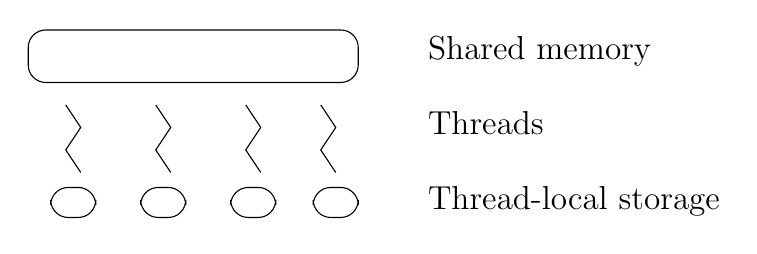
\begin{tikzpicture}[y=-1cm,scale=0.6]

% objects at depth 50:
\draw[rounded corners=6.3bp,black] (8.41375,1.42875) rectangle (1.42875,0.3175);
\draw[rounded corners=6.3bp,black] (2.8575,4.28625) rectangle (1.905,3.65125);
\draw[rounded corners=6.3bp,black] (4.7625,4.28625) rectangle (3.81,3.65125);
\draw[rounded corners=6.3bp,black] (6.6675,4.28625) rectangle (5.715,3.65125);
\draw[rounded corners=6.3bp,black] (8.41375,4.28625) rectangle (7.46125,3.65125);
\draw[black] (7.62,1.905) -- (7.9375,2.38125) -- (7.62,2.8575) -- (7.9375,3.33375);
\draw[black] (6.0325,1.905) -- (6.35,2.38125) -- (6.0325,2.8575) -- (6.35,3.33375);
\draw[black] (4.1275,1.905) -- (4.445,2.38125) -- (4.1275,2.8575) -- (4.445,3.33375);
\draw[black] (2.2225,1.905) -- (2.54,2.38125) -- (2.2225,2.8575) -- (2.54,3.33375);
\path (9.68375,2.54) node[text=black,anchor=base west] {\large{}Threads};
\path (9.68375,0.9525) node[text=black,anchor=base west] {\large{}Shared memory};
\path (9.68375,4.1275) node[text=black,anchor=base west] {\large{}Thread-local storage};

\end{tikzpicture}%

  \end{center}
  Program consists of {\em threads} of control.
  \begin{itemize}
  \item Can be created dynamically
  \item Each has private variables (e.g.~local)
  \item Each has shared variables (e.g.~heap)
  \item Communication through shared variables
  \item Coordinate by synchronizing on variables
  \item Examples: OpenMP, pthreads
  \end{itemize}
\end{frame}


\begin{frame}
  \frametitle{Shared memory dot product}
  
  Dot product of two $n$ vectors on $p \ll n$ processors:
  \begin{enumerate}
  \item Each CPU evaluates partial sum ($n/p$ elements, local)
  \item Everyone tallies partial sums
  \end{enumerate}
  Can we go home now?
\end{frame}


\begin{frame}
  \frametitle{Race condition}

  A {\em race condition}:
  \begin{itemize}
  \item Two threads access same variable, at least one write.
  \item Access are concurrent -- no ordering guarantees
    \begin{itemize}
    \item Could happen simultaneously!
    \end{itemize}
  \end{itemize}
  Need synchronization via lock or barrier.
\end{frame}


\begin{frame}[fragile]
  \frametitle{Race to the dot}

  Consider {\tt S += partial\_sum} on 2 CPU:
  \begin{itemize}
  \item P1: Load {\tt S}
  \item P1: Add {\tt partial\_sum}
  \item P2: Load {\tt S}
  \item P1: Store new {\tt S}
  \item P2: Add {\tt partial\_sum}
  \item P2: Store new {\tt S}
  \end{itemize}
\end{frame}

\begin{frame}
  \frametitle{Shared memory dot with locks}

  Solution: consider {\tt S += partial\_sum} a {\em critical section}
  \begin{itemize}
  \item Only one CPU at a time allowed in critical section
  \item Can violate invariants locally
  \item Enforce via a lock or mutex (mutual exclusion variable)
  \end{itemize}
  
  \vspace{5mm}
  Dot product with mutex:
  \begin{enumerate}
  \item Create global mutex {\tt l}
  \item Compute {\tt partial\_sum}
  \item Lock {\tt l}
  \item {S += partial\_sum}
  \item Unlock {\tt l}
  \end{enumerate}

\end{frame}


\begin{frame}
  \frametitle{Shared memory with barriers}
  
  \begin{itemize}
  \item Many codes have phases (e.g. time steps)
  \item Communication only needed at end of phases
  \item Idea: synchronize on end of phase with {\em barrier}
    \begin{itemize}
    \item More restrictive (less efficient?) than small locks
    \item Easier to think through!  (e.g. less chance of deadlocks)
    \end{itemize}
  \item Sometimes called {\em bulk synchronous programming}
  \end{itemize}

\end{frame}


\begin{frame}
  \frametitle{Shared memory machine model}

  \begin{itemize}
  \item Processors and memories talk through a bus
  \item Symmetric Multiprocessor (SMP)
  \item Hard to scale to lots of processors (think $\leq 32$)
    \begin{itemize}
      \item Bus becomes bottleneck
      \item {\em Cache coherence} is a pain
    \end{itemize}
  \item Example: Quad-core chips on cluster
  \end{itemize}
\end{frame}


\begin{frame}
  \frametitle{Multithreaded processor machine}
  
  \begin{itemize}
  \item May have more threads than processors!
  \item Can switch threads on long latency ops
    \begin{itemize}
    \item Cray MTA was an extreme example
    \end{itemize}
  \item Similar to {\em hyperthreading}
    \begin{itemize}
    \item But hyperthreading doesn't switch -- just schedules multiple
      threads onto same CPU functional units
    \end{itemize}
  \end{itemize}
\end{frame}


\begin{frame}
  \frametitle{Distributed shared memory}
 
  \begin{itemize}
  \item Non-Uniform Memory Access (NUMA)
  \item Can {\em logically} share memory while {\em physically} distributing
  \item Any processor can access any address
  \item Cache coherence is still a pain
  \item Example: SGI Origin (or multiprocessor nodes on cluster)
  \end{itemize}
\end{frame}


\begin{frame}
  \frametitle{Message-passing programming model}

  \begin{center}
    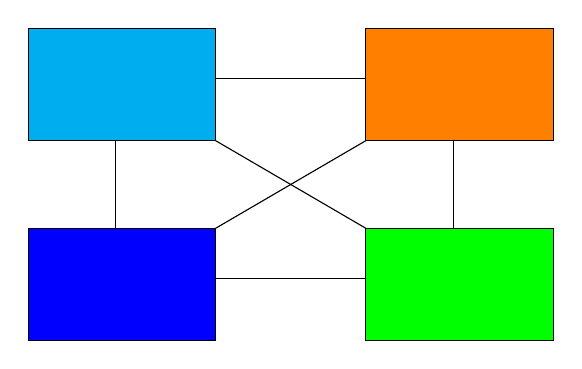
\begin{tikzpicture}[y=-1cm]

% objects at depth 50:
\draw[black,fill=blue] (2.54,3.96875) rectangle (4.92125,5.3975);
\draw[black,fill=green] (6.82625,3.96875) rectangle (9.2075,5.3975);
\draw[black,fill=orange] (6.82625,1.42875) rectangle (9.2075,2.8575);
\draw[black,fill=cyan] (2.54,1.42875) rectangle (4.92125,2.8575);
\draw[black] (4.92125,2.06375) -- (6.82625,2.06375);
\draw[black] (4.92125,4.60375) -- (6.82625,4.60375);
\draw[black] (3.65125,2.8575) -- (3.65125,3.96875);
\draw[black] (7.9375,2.8575) -- (7.9375,3.96875);
\draw[black] (4.92125,2.8575) -- (6.82625,3.96875);
\draw[black] (4.92125,3.96875) -- (6.82625,2.8575);

\end{tikzpicture}%

  \end{center}
  \begin{itemize}
  \item Collection of named processes
  \item Data is {\em partitioned}
  \item Communication by send/receive of explicit message
  \item Lingua franca: MPI (Message Passing Interface)
  \end{itemize}
\end{frame}


\begin{frame}
  \frametitle{Message passing dot product: v1}

  \begin{minipage}{0.45\textwidth}
    Processor 1:
    \begin{enumerate}
    \item Partial sum s1
    \item Send s1 to P2
    \item Receive s2 from P2
    \item s = s1 + s2
    \end{enumerate}
  \end{minipage}
  \begin{minipage}{0.45\textwidth}
    Processor 2:
    \begin{enumerate}
    \item Partial sum s2
    \item Send s2 to P1
    \item Receive s1 from P1
    \item s = s1 + s2
    \end{enumerate}
  \end{minipage}

  \vspace{1cm}
  What could go wrong?  Think of phones vs letters...

\end{frame}


\begin{frame}
  \frametitle{Message passing dot product: v1}

  \begin{minipage}{0.45\textwidth}
    Processor 1:
    \begin{enumerate}
    \item Partial sum s1
    \item Send s1 to P2
    \item Receive s2 from P2
    \item s = s1 + s2
    \end{enumerate}
  \end{minipage}
  \begin{minipage}{0.45\textwidth}
    Processor 2:
    \begin{enumerate}
    \item Partial sum s2
    \item Receive s1 from P1
    \item Send s2 to P1
    \item s = s1 + s2
    \end{enumerate}
  \end{minipage}

  \vspace{1cm}
  Better, but what if more than two processors?

\end{frame}


\begin{frame}
  \frametitle{MPI: the de facto standard}

  \begin{itemize}
  \item Pro: {\em Portability}
  \item Con: least-common-denominator for mid 80s
  \end{itemize}
  The ``assembly language'' (or C?) of parallelism... \\
  \hspace{5mm} but, alas, assembly language can be high performance.

\end{frame}


\begin{frame}
  \frametitle{Distributed memory machines}
  
  \begin{itemize}
  \item Each node has local memory
    \begin{itemize}
    \item ... and no direct access to memory on other nodes
    \end{itemize}
  \item Nodes communicate via network interface
  \item Example: our cluster!
  \item Other examples: IBM SP, Cray T3E
  \end{itemize}
\end{frame}

\begin{frame}
  \frametitle{The story so far}

  \begin{itemize}
  \item Even {\em serial} performance is a complicated function of
        the underlying architecture and memory system.  We need to
        understand these effects in order to design data structures
        and algorithms that are fast on modern machines.  Good
        serial performance is the basis for good parallel performance.
  \item {\em Parallel} performance is additionally complicated by
        communication and synchronization overheads, and by how
        much parallel work is available.  If a small fraction of the
        work is completely serial, Amdahl's law bounds the speedup,
        independent of the number of processors.
  \item We have discussed serial architecture and some of the basics
        of parallel machine models and programming models.
  \item Now we want to describe how to think about the shape of
        parallel algorithms for some scientific applications.
  \end{itemize}
\end{frame}

\begin{frame}
  \frametitle{Reminder: what do we want?}

  \begin{itemize}
  \item High-level: solve big problems fast
  \item Start with good {\em serial} performance
  \item Given $p$ processors, could then ask for
    \begin{itemize}
    \item Good {\em speedup}: $p^{-1}$ times serial time
    \item Good {\em scaled speedup}: $p$ times the work in same time
    \end{itemize}
  \item Easiest to get good speedup from cruddy serial code!
  \end{itemize}
\end{frame}


\begin{frame}
  \frametitle{Parallelism and locality}

  \begin{itemize}
  \item Real world exhibits {\em parallelism} and {\em locality}
    \begin{itemize}
    \item Particles, people, etc function independently
    \item Nearby objects interact more strongly than distant ones
    \item Can often simplify dependence on distant objects
    \end{itemize}
  \item Can get more parallelism / locality through model
    \begin{itemize}
    \item Limited range of dependency between adjacent time steps
    \item Can neglect or approximate far-field effects
    \end{itemize}
  \item Often get parallism at multiple levels
    \begin{itemize}
    \item Hierarchical circuit simulation
    \item Interacting models for climate
    \item Parallelizing individual experiments in MC or optimization
    \end{itemize}
  \end{itemize}
\end{frame}


\begin{frame}
  \frametitle{Basic styles of simulation}

  \begin{itemize}
  \item Discrete event systems (continuous or discrete time)
    \begin{itemize}
    \item Game of life, logic-level circuit simulation
    \item Network simulation
    \end{itemize}
  \item Particle systems
    \begin{itemize}
    \item Billiards, electrons, galaxies, ...
    \item Ants, cars, ...?
    \end{itemize}
  \item Lumped parameter models (ODEs)
    \begin{itemize}
    \item Circuits (SPICE), structures, chemical kinetics
    \end{itemize}
  \item Distributed parameter models (PDEs / integral equations)
    \begin{itemize}
    \item Heat, elasticity, electrostatics, ...
    \end{itemize}
  \end{itemize}
  Often more than one type of simulation appropriate. \\
  Sometimes more than one at a time!

\end{frame}

\end{document}
% This is as far as we actually got

\begin{frame}
  \frametitle{Discrete events}

  Basic setup:
  \begin{itemize}
  \item Finite set of variables, updated via transition function
  \item {\em Synchronous} case: finite state machine
  \item {\em Asynchronous} case: event-driven simulation
  \item Synchronous example: Game of Life
  \end{itemize}

  \vspace{5mm}
  Nice starting point --- no discretization concerns!
\end{frame}


\begin{frame}
  \frametitle{Game of Life}

  \begin{center}
    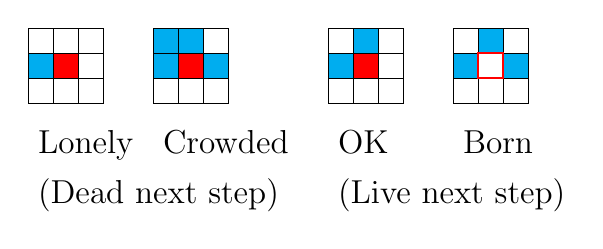
\begin{tikzpicture}[y=-1cm]

% objects at depth 50:
\draw[black] (0.635,0.635) rectangle (1.5875,1.5875);
\path[draw=black,fill=red] (0.9525,0.9525) rectangle (1.27,1.27);
\draw[black] (0.635,0.9525) -- (1.5875,0.9525);
\draw[black] (0.635,1.27) -- (1.5875,1.27);
\draw[black] (0.9525,0.635) -- (0.9525,1.5875);
\draw[black] (1.27,0.635) -- (1.27,1.5875);
\draw[black] (2.2225,0.635) rectangle (3.175,1.5875);
\path[draw=black,fill=red] (2.54,0.9525) rectangle (2.8575,1.27);
\draw[black] (2.2225,0.9525) -- (3.175,0.9525);
\draw[black] (2.2225,1.27) -- (3.175,1.27);
\draw[black] (2.54,0.635) -- (2.54,1.5875);
\draw[black] (2.8575,0.635) -- (2.8575,1.5875);
\draw[black] (4.445,0.635) rectangle (5.3975,1.5875);
\path[draw=black,fill=red] (4.7625,0.9525) rectangle (5.08,1.27);
\draw[black] (4.445,0.9525) -- (5.3975,0.9525);
\draw[black] (4.445,1.27) -- (5.3975,1.27);
\draw[black] (4.7625,0.635) -- (4.7625,1.5875);
\draw[black] (5.08,0.635) -- (5.08,1.5875);
\draw[black] (6.0325,0.635) rectangle (6.985,1.5875);
\draw[black] (6.0325,0.9525) -- (6.985,0.9525);
\draw[black] (6.35,0.635) -- (6.35,1.5875);
\draw[black] (6.35,0.9525) rectangle (6.6675,1.27);
\draw[black] (6.0325,1.27) -- (6.985,1.27);
\draw[black] (6.6675,0.635) -- (6.6675,1.5875);
\path[draw=black,fill=cyan] (2.54,0.9525) rectangle (2.2225,1.27);
\path[draw=black,fill=cyan] (2.8575,0.635) rectangle (2.54,0.9525);
\path[draw=black,fill=cyan] (2.54,0.635) rectangle (2.2225,0.9525);
\path[draw=black,fill=cyan] (3.175,0.9525) rectangle (2.8575,1.27);
\path[draw=black,fill=cyan] (4.7625,0.9525) rectangle (4.445,1.27);
\path[draw=black,fill=cyan] (5.08,0.635) rectangle (4.7625,0.9525);
\path[draw=black,fill=cyan] (6.6675,0.635) rectangle (6.35,0.9525);
\path[draw=black,fill=cyan] (6.35,0.9525) rectangle (6.0325,1.27);
\path[draw=black,fill=cyan] (6.985,0.9525) rectangle (6.6675,1.27);
\path[draw=black,fill=cyan] (0.9525,0.9525) rectangle (0.635,1.27);
\draw[semithick,red] (6.6675,0.9525) rectangle (6.35,1.27);
\path (0.635,2.2225) node[text=black,anchor=base west] {\large{}Lonely};
\path (2.2225,2.2225) node[text=black,anchor=base west] {\large{}Crowded};
\path (4.445,2.2225) node[text=black,anchor=base west] {\large{}OK};
\path (6.0325,2.2225) node[text=black,anchor=base west] {\large{}Born};
\path (0.635,2.8575) node[text=black,anchor=base west] {\large{}(Dead next step)};
\path (4.445,2.8575) node[text=black,anchor=base west] {\large{}(Live next step)};

\end{tikzpicture}%

  \end{center}

  Game of Life (John Conway):
  \begin{enumerate}
  \item Live cell dies with < 2 live neighbors
  \item Live cell dies with > 3 live neighbors
  \item Live cell lives with 2--3 live neighbors
  \item Dead cell becomes live with exactly 3 live neighbors
  \end{enumerate}
\end{frame}

\begin{frame}
  \frametitle{Game of Life}

  \begin{center}
    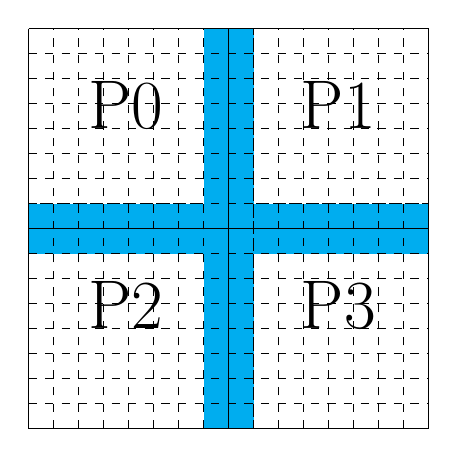
\begin{tikzpicture}[y=-1cm]

% objects at depth 60:
\path[draw=black,fill=cyan,dashed] (1.27,3.4925) rectangle (6.35,4.1275);
\path[draw=black,fill=cyan,dashed] (3.4925,6.35) rectangle (4.1275,1.27);

% objects at depth 50:
\draw[dashed,black] (1.27,4.1275) -- (6.35,4.1275);
\draw[dashed,black] (1.27,4.445) -- (6.35,4.445);
\draw[dashed,black] (1.27,4.7625) -- (6.35,4.7625);
\draw[dashed,black] (1.27,5.08) -- (6.35,5.08);
\draw[dashed,black] (1.27,5.3975) -- (6.35,5.3975);
\draw[dashed,black] (1.27,5.715) -- (6.35,5.715);
\draw[dashed,black] (1.27,6.0325) -- (6.35,6.0325);
\draw[dashed,black] (1.27,3.4925) -- (6.35,3.4925);
\draw[dashed,black] (1.27,3.175) -- (6.35,3.175);
\draw[dashed,black] (1.27,2.8575) -- (6.35,2.8575);
\draw[dashed,black] (1.27,1.905) -- (6.35,1.905);
\draw[dashed,black] (1.27,1.5875) -- (6.35,1.5875);
\draw[dashed,black] (1.5875,6.35) -- (1.5875,1.27);
\draw[dashed,black] (2.54,6.35) -- (2.54,1.27);
\draw[dashed,black] (2.8575,6.35) -- (2.8575,1.27);
\draw[dashed,black] (3.175,6.35) -- (3.175,1.27);
\draw[dashed,black] (3.4925,6.35) -- (3.4925,1.27);
\draw[dashed,black] (4.1275,6.35) -- (4.1275,1.27);
\draw[dashed,black] (4.445,6.35) -- (4.445,1.27);
\draw[dashed,black] (4.7625,6.35) -- (4.7625,1.27);
\draw[dashed,black] (5.08,6.35) -- (5.08,1.27);
\draw[dashed,black] (5.3975,6.35) -- (5.3975,1.27);
\draw[dashed,black] (5.715,6.35) -- (5.715,1.27);
\draw[dashed,black] (6.0325,6.35) -- (6.0325,1.27);
\draw[semithick,black] (6.35,1.27) -- (6.35,6.35);
\draw[semithick,black] (1.27,1.27) -- (6.35,1.27);
\draw[semithick,black] (1.27,1.27) -- (1.27,6.35);
\draw[semithick,black] (1.27,6.35) -- (6.35,6.35);
\draw[semithick,black] (3.81,1.27) -- (3.81,6.35);
\draw[semithick,black] (1.27,3.81) -- (6.35,3.81);
\draw[dashed,black] (1.27,2.54) -- (6.35,2.54);
\draw[dashed,black] (1.905,6.35) -- (1.905,1.27);
\draw[dashed,black] (1.27,2.2225) -- (6.35,2.2225);
\draw[dashed,black] (2.2225,6.35) -- (2.2225,1.27);
\path (1.905,2.54) node[text=black,anchor=base west] {\Huge{}P0};
\path (4.60375,2.54) node[text=black,anchor=base west] {\Huge{}P1};
\path (1.905,5.08) node[text=black,anchor=base west] {\Huge{}P2};
\path (4.60375,5.08) node[text=black,anchor=base west] {\Huge{}P3};

\end{tikzpicture}%

  \end{center}

  Easy to parallelize by {\em domain decomposition}.
  \begin{itemize}
  \item Update work involves {\em volume} of subdomains
  \item Communication per step on {\em surface} (cyan)
  \end{itemize}

\end{frame}


\begin{frame}
  \frametitle{Game of Life: Pioneers and Settlers}

  What if pattern is ``dilute''?
  \begin{itemize}
  \item Few or no live cells at surface at each step
  \item Think of live cell at a surface as an ``event''
  \item Only communicate events!
    \begin{itemize}
    \item This is {\em asynchronous}
    \item Harder with message passing --- when do you receive?
    \end{itemize}
  \end{itemize}

\end{frame}


\begin{frame}
  \frametitle{Asynchronous Game of Life}

  How do we manage events?
  \begin{itemize}
  \item Could be {\em speculative} --- assume no communication across boundary
    for many steps, back up if needed
  \item Or {\em conservative} --- wait whenever communication possible
    \begin{itemize}
    \item possible $\not \equiv$ guaranteed!
    \item Deadlock: everyone waits for everyone else to send data
    \item Can get around this with NULL messages
    \end{itemize}
  \end{itemize}
  
  \vspace{3mm}
  How do we manage load balance?
  \begin{itemize}
  \item No need to simulate quiescent parts of the game!
  \item Maybe dynamically assign smaller blocks to processors?
  \end{itemize}

\end{frame}


\begin{frame}
  \frametitle{Particle simulation}

  Particles move via Newton ($F = ma$), with
  \begin{itemize}
  \item External forces: ambient gravity, currents, etc.
  \item Local forces: collisions, Van der Waals ($1/r^6$), etc.
  \item Far-field forces: gravity and electrostatics ($1/r^2$), etc.
    \begin{itemize}
    \item Simple approximations often apply (Saint-Venant)
    \end{itemize}
  \end{itemize}
\end{frame}


\begin{frame}
  \frametitle{A forced example}

  Example force:
  \[
    f_i = \sum_j Gm_i m_j
      \frac{(x_j-x_i)}{r_{ij}^3}
      \left(1 - \left(\frac{a}{r_{ij}}\right)^{4} \right), \qquad
      r_{ij} = \|x_i-x_j\|
  \]
  \begin{itemize}
  \item Long-range attractive force ($r^{-2}$)
  \item Short-range repulsive force ($r^{-6}$)
  \item Go from attraction to repulsion at radius $a$
  \end{itemize}

\end{frame}


\begin{frame}[fragile]
  \frametitle{A simple serial simulation}

  In \textsc{Matlab}, we can write
\begin{verbatim}
  npts = 100;
  t = linspace(0, tfinal, npts);
  [tout, xyv] = ode113(@fnbody, ...
                t, [x; v], [], m, g);
  xout = xyv(:,1:length(x))';
\end{verbatim}
  ... but I can't call {\tt ode113} in C in parallel (or can I?)

\end{frame}


\begin{frame}[fragile]
  \frametitle{A simple serial simulation}

  Maybe a fixed step leapfrog will do?
\begin{verbatim}
  npts = 100;
  steps_per_pt = 10;
  dt = tfinal/(steps_per_pt*(npts-1));
  xout = zeros(2*n, npts);
  xout(:,1) = x;
  for i = 1:npts-1
    for ii = 1:steps_per_pt
      x = x + v*dt;
      a = fnbody(x, m, g);
      v = v + a*dt;
    end
    xout(:,i+1) = x;
  end
\end{verbatim}

\end{frame}


\begin{frame}
  \frametitle{Plotting particles}

  \begin{center}
    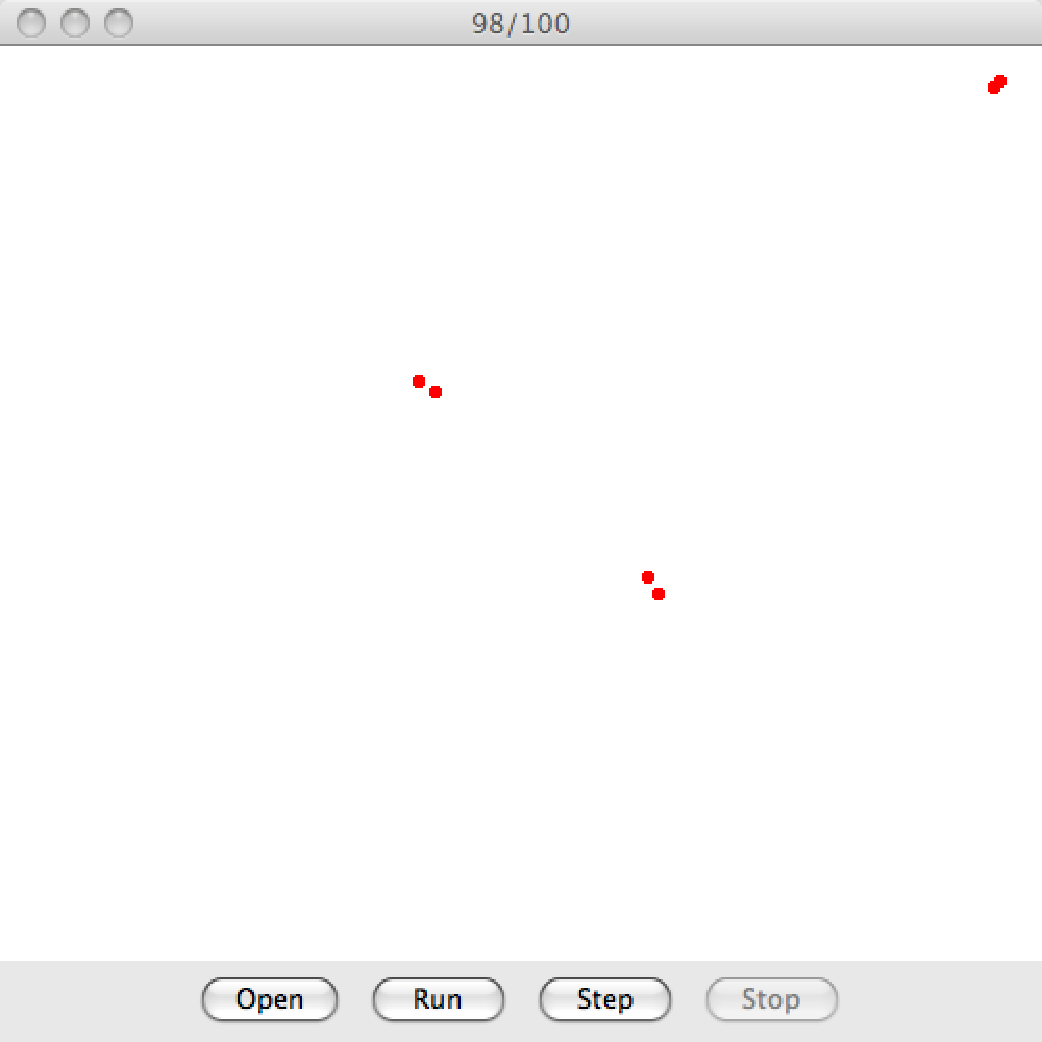
\includegraphics[width=0.7\textwidth]{lec05bouncy.pdf}
  \end{center}
\end{frame}



\begin{frame}
  \frametitle{Pondering particles}
  
  \begin{itemize}
  \item Where do particles ``live'' (esp.~in distributed memory)?
    \begin{itemize}
    \item Decompose in space?  By particle number?
    \item What about clumping?
    \end{itemize}
  \item How are long-range force computations organized?
  \item How are short-range force computations organized?
  \item How is force computation load balanced?
  \item What are the boundary conditions?
  \item How are potential singularities handled?
  \item What integrator is used?  What step control?
  \end{itemize}
\end{frame}


\begin{frame}
  \frametitle{External forces}

  Simplest case: no particle interactions.
  \begin{itemize}
    \item Embarrassingly parallel (like Monte Carlo)!
    \item Could just split particles evenly across processors
    \item Is it that easy?
      \begin{itemize}
      \item Maybe some trajectories need short time steps?
      \item Even with MC, load balance may not be entirely trivial.
      \end{itemize}
  \end{itemize}
\end{frame}


\begin{frame}
  \frametitle{Local forces}
  
  \begin{center}
    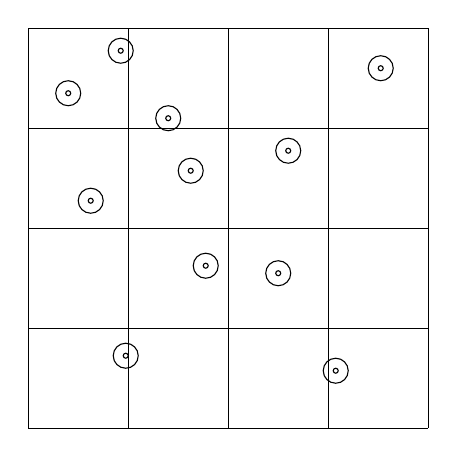
\begin{tikzpicture}[y=-1cm]

% objects at depth 50:
\draw[black] (2.44475,1.55575) circle (0.15875cm);
\draw[black] (2.44475,1.55575) circle (0.03175cm);
\draw[black] (1.778,2.0955) circle (0.15875cm);
\draw[black] (1.778,2.0955) circle (0.03175cm);
\draw[black] (3.33375,3.07975) circle (0.15875cm);
\draw[black] (3.33375,3.07975) circle (0.03175cm);
\draw[black] (3.048,2.413) circle (0.15875cm);
\draw[black] (3.048,2.413) circle (0.03175cm);
\draw[black] (2.06375,3.46075) circle (0.15875cm);
\draw[black] (2.06375,3.46075) circle (0.03175cm);
\draw[black] (3.52425,4.28625) circle (0.15875cm);
\draw[black] (3.52425,4.28625) circle (0.03175cm);
\draw[black] (4.445,4.3815) circle (0.15875cm);
\draw[black] (4.445,4.3815) circle (0.03175cm);
\draw[black] (4.572,2.82575) circle (0.15875cm);
\draw[black] (4.572,2.82575) circle (0.03175cm);
\draw[black] (5.74675,1.778) circle (0.15875cm);
\draw[black] (5.74675,1.778) circle (0.03175cm);
\draw[black] (2.50825,5.42925) circle (0.15875cm);
\draw[black] (2.50825,5.42925) circle (0.03175cm);
\draw[black] (5.17525,5.61975) circle (0.15875cm);
\draw[black] (5.17525,5.61975) circle (0.03175cm);
\draw[black] (1.27,1.27) -- (1.27,6.35);
\draw[black] (2.54,1.27) -- (2.54,6.35);
\draw[black] (3.81,1.27) -- (3.81,6.35);
\draw[black] (5.08,1.27) -- (5.08,6.35);
\draw[black] (6.35,1.27) -- (6.35,6.35);
\draw[black] (1.27,1.27) -- (6.35,1.27);
\draw[black] (1.27,2.54) -- (6.35,2.54);
\draw[black] (1.27,3.81) -- (6.35,3.81);
\draw[black] (1.27,5.08) -- (6.35,5.08);
\draw[black] (1.27,6.35) -- (6.35,6.35);

\end{tikzpicture}%

  \end{center}
  \begin{itemize}
  \item Simplest all-pairs check is $O(n^2)$ (expensive)
  \item Or only check close pairs (via binning, quadtrees?)
  \item Communication required for pairs checked
  \item Usual model: domain decomposition
  \end{itemize}

\end{frame}


\begin{frame}
  \frametitle{Local forces: Communication}

  \begin{center}
    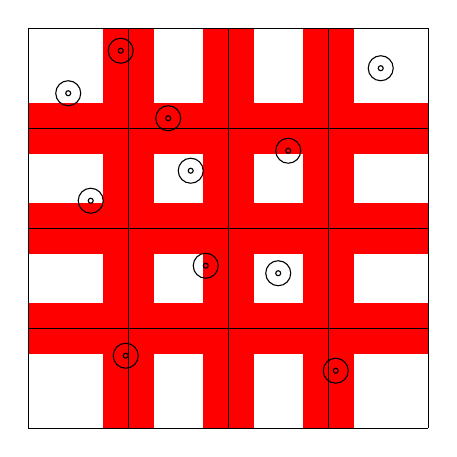
\begin{tikzpicture}[y=-1cm]

% objects at depth 60:
\filldraw[red] (2.2225,1.27) rectangle (2.8575,6.35);
\filldraw[red] (3.4925,1.27) rectangle (4.1275,6.35);
\filldraw[red] (4.7625,1.27) rectangle (5.3975,6.35);
\filldraw[red] (1.27,5.3975) rectangle (6.35,4.7625);
\filldraw[red] (1.27,4.1275) rectangle (6.35,3.4925);
\filldraw[red] (1.27,2.8575) rectangle (6.35,2.2225);

% objects at depth 50:
\draw[black] (2.44475,1.55575) circle (0.15875cm);
\draw[black] (2.44475,1.55575) circle (0.03175cm);
\draw[black] (1.778,2.0955) circle (0.15875cm);
\draw[black] (1.778,2.0955) circle (0.03175cm);
\draw[black] (3.33375,3.07975) circle (0.15875cm);
\draw[black] (3.33375,3.07975) circle (0.03175cm);
\draw[black] (3.048,2.413) circle (0.15875cm);
\draw[black] (3.048,2.413) circle (0.03175cm);
\draw[black] (2.06375,3.46075) circle (0.15875cm);
\draw[black] (2.06375,3.46075) circle (0.03175cm);
\draw[black] (3.52425,4.28625) circle (0.15875cm);
\draw[black] (3.52425,4.28625) circle (0.03175cm);
\draw[black] (4.445,4.3815) circle (0.15875cm);
\draw[black] (4.445,4.3815) circle (0.03175cm);
\draw[black] (4.572,2.82575) circle (0.15875cm);
\draw[black] (4.572,2.82575) circle (0.03175cm);
\draw[black] (5.74675,1.778) circle (0.15875cm);
\draw[black] (5.74675,1.778) circle (0.03175cm);
\draw[black] (2.50825,5.42925) circle (0.15875cm);
\draw[black] (2.50825,5.42925) circle (0.03175cm);
\draw[black] (5.17525,5.61975) circle (0.15875cm);
\draw[black] (5.17525,5.61975) circle (0.03175cm);
\draw[black] (1.27,1.27) -- (1.27,6.35);
\draw[black] (2.54,1.27) -- (2.54,6.35);
\draw[black] (3.81,1.27) -- (3.81,6.35);
\draw[black] (5.08,1.27) -- (5.08,6.35);
\draw[black] (6.35,1.27) -- (6.35,6.35);
\draw[black] (1.27,1.27) -- (6.35,1.27);
\draw[black] (1.27,2.54) -- (6.35,2.54);
\draw[black] (1.27,3.81) -- (6.35,3.81);
\draw[black] (1.27,5.08) -- (6.35,5.08);
\draw[black] (1.27,6.35) -- (6.35,6.35);

\end{tikzpicture}%

  \end{center}

  Minimize communication:
  \begin{itemize}
  \item Send particles that might affect a neighbor ``soon''
  \item Trade extra computation against communication
  \item Want low surface area-to-volume ratios on domains
  \end{itemize}
  
\end{frame}



\begin{frame}
  \frametitle{Local forces: Load balance}

  \begin{center}
    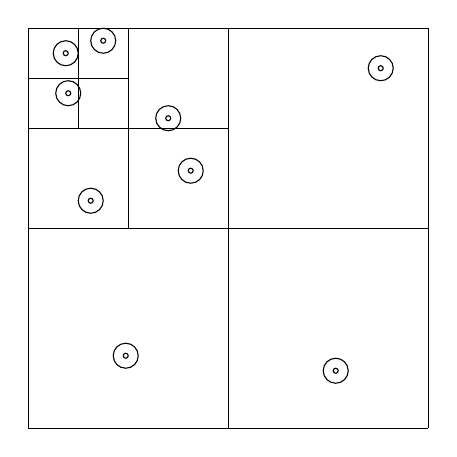
\begin{tikzpicture}[y=-1cm]

% objects at depth 50:
\draw[black] (1.778,2.0955) circle (0.15875cm);
\draw[black] (1.778,2.0955) circle (0.03175cm);
\draw[black] (3.33375,3.07975) circle (0.15875cm);
\draw[black] (3.33375,3.07975) circle (0.03175cm);
\draw[black] (3.048,2.413) circle (0.15875cm);
\draw[black] (3.048,2.413) circle (0.03175cm);
\draw[black] (2.06375,3.46075) circle (0.15875cm);
\draw[black] (2.06375,3.46075) circle (0.03175cm);
\draw[black] (5.74675,1.778) circle (0.15875cm);
\draw[black] (5.74675,1.778) circle (0.03175cm);
\draw[black] (2.50825,5.42925) circle (0.15875cm);
\draw[black] (2.50825,5.42925) circle (0.03175cm);
\draw[black] (5.17525,5.61975) circle (0.15875cm);
\draw[black] (5.17525,5.61975) circle (0.03175cm);
\draw[black] (1.74625,1.5875) circle (0.15875cm);
\draw[black] (1.74625,1.5875) circle (0.03175cm);
\draw[black] (2.2225,1.42875) circle (0.15875cm);
\draw[black] (2.2225,1.42875) circle (0.03175cm);
\draw[black] (1.27,1.27) -- (1.27,6.35);
\draw[black] (2.54,1.27) -- (2.54,3.81);
\draw[black] (3.81,1.27) -- (3.81,6.35);
\draw[black] (6.35,1.27) -- (6.35,6.35);
\draw[black] (1.27,1.27) -- (6.35,1.27);
\draw[black] (1.27,2.54) -- (3.81,2.54);
\draw[black] (1.27,3.81) -- (6.35,3.81);
\draw[black] (1.27,6.35) -- (6.35,6.35);
\draw[black] (1.27,1.905) -- (2.54,1.905);
\draw[black] (1.905,1.27) -- (1.905,2.54);

\end{tikzpicture}%

  \end{center}

  \begin{itemize}
  \item Are particles evenly distributed?
  \item Do particles remain evenly distributed?
  \item Can divide space unevenly (e.g.~quadtree/octtree)
  \end{itemize}
  
\end{frame}


\begin{frame}
  \frametitle{Far-field forces}

  \begin{center}
    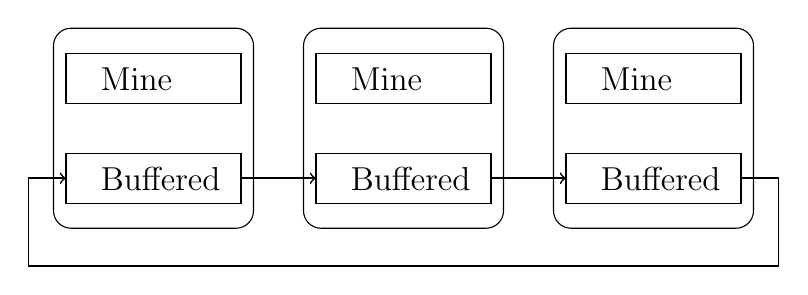
\begin{tikzpicture}[y=-1cm]

% objects at depth 50:
\draw[rounded corners=6.3bp,black] (5.08,5.08) rectangle (2.54,2.54);
\draw[black] (2.69875,2.8575) rectangle (4.92125,3.4925);
\draw[black] (2.69875,4.1275) rectangle (4.92125,4.7625);
\path (3.01625,3.33375) node[text=black,anchor=base west] {\large{}Mine};
\path (3.01625,4.60375) node[text=black,anchor=base west] {\large{}Buffered};
\draw[rounded corners=6.3bp,black] (8.255,5.08) rectangle (5.715,2.54);
\draw[black] (5.87375,2.8575) rectangle (8.09625,3.4925);
\draw[black] (5.87375,4.1275) rectangle (8.09625,4.7625);
\path (6.19125,3.33375) node[text=black,anchor=base west] {\large{}Mine};
\path (6.19125,4.60375) node[text=black,anchor=base west] {\large{}Buffered};
\draw[rounded corners=6.3bp,black] (11.43,5.08) rectangle (8.89,2.54);
\draw[black] (9.04875,2.8575) rectangle (11.27125,3.4925);
\draw[black] (9.04875,4.1275) rectangle (11.27125,4.7625);
\path (9.36625,3.33375) node[text=black,anchor=base west] {\large{}Mine};
\path (9.36625,4.60375) node[text=black,anchor=base west] {\large{}Buffered};
\draw[->,semithick,black] (4.92125,4.445) -- (5.87375,4.445);
\draw[->,semithick,black] (8.09625,4.445) -- (9.04875,4.445);
\draw[->,semithick,black] (11.27125,4.445) -- (11.7475,4.445) -- (11.7475,5.55625) -- (2.2225,5.55625) -- (2.2225,4.445) -- (2.69875,4.445);

\end{tikzpicture}%

  \end{center}

  \begin{itemize}
  \item Every particle affects every other particle
  \item All-to-all communication required
    \begin{itemize}
    \item Overlap communication with computation
    \item Poor memory scaling if everyone keeps everything!
    \end{itemize}
  \item Idea: pass particles in a round-robin manner
  \end{itemize}
\end{frame}


\begin{frame}[fragile]
  \frametitle{Passing particles for far-field forces}

  \begin{center}
    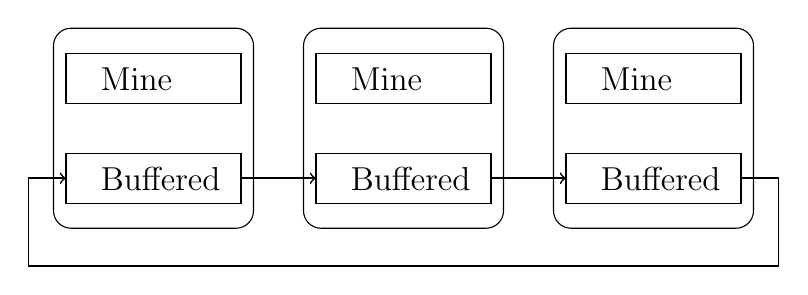
\begin{tikzpicture}[y=-1cm]

% objects at depth 50:
\draw[rounded corners=6.3bp,black] (5.08,5.08) rectangle (2.54,2.54);
\draw[black] (2.69875,2.8575) rectangle (4.92125,3.4925);
\draw[black] (2.69875,4.1275) rectangle (4.92125,4.7625);
\path (3.01625,3.33375) node[text=black,anchor=base west] {\large{}Mine};
\path (3.01625,4.60375) node[text=black,anchor=base west] {\large{}Buffered};
\draw[rounded corners=6.3bp,black] (8.255,5.08) rectangle (5.715,2.54);
\draw[black] (5.87375,2.8575) rectangle (8.09625,3.4925);
\draw[black] (5.87375,4.1275) rectangle (8.09625,4.7625);
\path (6.19125,3.33375) node[text=black,anchor=base west] {\large{}Mine};
\path (6.19125,4.60375) node[text=black,anchor=base west] {\large{}Buffered};
\draw[rounded corners=6.3bp,black] (11.43,5.08) rectangle (8.89,2.54);
\draw[black] (9.04875,2.8575) rectangle (11.27125,3.4925);
\draw[black] (9.04875,4.1275) rectangle (11.27125,4.7625);
\path (9.36625,3.33375) node[text=black,anchor=base west] {\large{}Mine};
\path (9.36625,4.60375) node[text=black,anchor=base west] {\large{}Buffered};
\draw[->,semithick,black] (4.92125,4.445) -- (5.87375,4.445);
\draw[->,semithick,black] (8.09625,4.445) -- (9.04875,4.445);
\draw[->,semithick,black] (11.27125,4.445) -- (11.7475,4.445) -- (11.7475,5.55625) -- (2.2225,5.55625) -- (2.2225,4.445) -- (2.69875,4.445);

\end{tikzpicture}%

  \end{center}

\begin{verbatim}
copy local particles to current buf
for phase = 1:p
  send current buf to rank+1 (mod p)
  recv next buf from rank-1 (mod p) 
  interact local particles with current buf
  swap current buf with next buf
end
\end{verbatim}
\end{frame}



\begin{frame}
  \frametitle{Passing particles for far-field forces}

  Suppose $n = N/p$ particles in buffer.  At each phase
  \begin{align*}
    t_{\mathrm{comm}} & \approx \alpha + \beta n \\
    t_{\mathrm{comp}} & \approx \gamma n^2
  \end{align*}
  So we can mask communication with computation if
  \[
  n \geq
    \frac{1}{2\gamma} \left( \beta + \sqrt{\beta^2 + 4 \alpha \gamma} \right)
    > \frac{\beta}{\gamma}
  \]

  \vspace{4mm}
  More efficient serial code \\
  $\implies$ larger $n$ needed to mask communication! \\
  $\implies$ worse speed-up as $p$ gets larger (fixed $N$) \\
  but scaled speed-up ($n$ fixed) remains unchanged.

  \vspace{4mm}
  This analysis neglects overhead term in LogP.
  
\end{frame}


\begin{frame}
  \frametitle{Far-field forces: particle-mesh methods}

  Consider $r^{-2}$ electrostatic potential interaction
  \begin{itemize}
  \item Enough charges looks like a continuum!
  \item Poisson equation maps charge distribution to potential
  \item Use fast Poisson solvers for regular grids (FFT, multigrid)
  \item Approximation depends on mesh and particle density
  \item Can clean up leading part of approximation error
  \end{itemize}

\end{frame}


\begin{frame}
  \frametitle{Far-field forces: particle-mesh methods}

  \begin{center}
    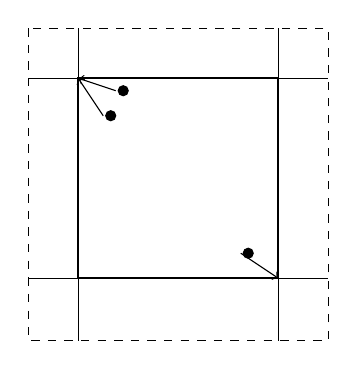
\begin{tikzpicture}[y=-1cm]

% objects at depth 50:
\filldraw[black] (4.3815,3.96875) circle (0.0635cm);
\filldraw[black] (5.969,6.0325) circle (0.0635cm);
\filldraw[black] (4.22275,4.28625) circle (0.0635cm);
\draw[black] (3.81,3.175) -- (3.81,7.14375);
\draw[black] (6.35,3.175) -- (6.35,7.14375);
\draw[black] (3.175,6.35) -- (6.985,6.35);
\draw[->,black] (4.1275,4.28625) -- (3.81,3.81);
\draw[semithick,black] (3.81,3.81) rectangle (6.35,6.35);
\draw[black] (3.175,3.81) -- (6.985,3.81);
\draw[->,black] (4.28625,3.96875) -- (3.81,3.81);
\draw[->,black] (5.87375,6.0325) -- (6.35,6.35);
\draw[dashed,black] (3.175,3.175) rectangle (6.985,7.14375);

\end{tikzpicture}%

  \end{center}
  
  \begin{itemize}
  \item Map particles to mesh points (multiple strategies)
  \item Solve potential PDE on mesh
  \item Interpolate potential to particles
  \item Add correction term -- acts like local force
  \end{itemize}

\end{frame}


\begin{frame}
  \frametitle{Far-field forces: tree methods}

  \begin{center}
%    \includegraphics[width=\textwidth]{lec04tree.pdf}
    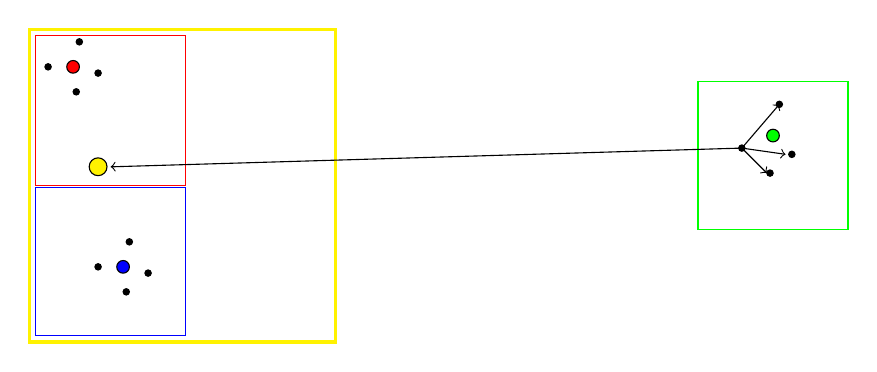
\begin{tikzpicture}[y=-1cm,scale=0.5]

% objects at depth 50:
\filldraw[black] (2.30293,1.42875) circle (0.08043cm);
\filldraw[black] (2.8575,0.9525) circle (0.08043cm);
\filldraw[black] (2.38125,0.15875) circle (0.08043cm);
\filldraw[black] (1.5875,0.79375) circle (0.08043cm);
\path[draw=black,fill=red] (2.2225,0.79375) circle (0.16087cm);
\filldraw[black] (3.57293,6.50875) circle (0.08043cm);
\filldraw[black] (4.1275,6.0325) circle (0.08043cm);
\filldraw[black] (3.65125,5.23875) circle (0.08043cm);
\filldraw[black] (2.8575,5.87375) circle (0.08043cm);
\path[draw=black,fill=blue] (3.4925,5.87375) circle (0.16087cm);
\path[draw=black,fill=yellow] (2.8575,3.33163) circle (0.22648cm);
\filldraw[black] (19.92418,3.4925) circle (0.08043cm);
\filldraw[black] (20.47875,3.01625) circle (0.08043cm);
\filldraw[black] (19.20875,2.8575) circle (0.08043cm);
\filldraw[black] (20.16125,1.74625) circle (0.08043cm);
\path[draw=black,fill=green] (20.00038,2.54) circle (0.16087cm);
\draw[semithick,red] (1.27,0) rectangle (5.08,3.81);
\draw[semithick,blue] (1.27,3.8608) rectangle (5.08,7.62);
\draw[very thick,yellow] (1.11125,-0.15875) rectangle (8.89,7.77875);
\draw[semithick,green] (18.0975,1.16205) rectangle (21.9075,4.92125);
\draw[arrows=-to,black] (19.20875,2.8575) -- (3.175,3.33375);
\draw[arrows=-to,black] (19.20875,2.8575) -- (20.16125,1.74625);
\draw[arrows=-to,black] (19.20875,2.8575) -- (20.32,3.01625);
\draw[arrows=-to,black] (19.20875,2.8575) -- (19.84375,3.4925);

\end{tikzpicture}%

  \end{center}
  \begin{itemize}
  \item Distance simplifies things
    \begin{itemize}
    \item Andromeda looks like a point mass from here?
    \end{itemize}
  \item Build a tree, approximating descendants at each node
  \item Several variants: Barnes-Hut, FMM, Anderson's method
  \item More on this later in the semester
  \end{itemize}
\end{frame}


\begin{frame}
  \frametitle{Summary of particle example}

  \begin{itemize}
  \item Model: Continuous motion of particles
    \begin{itemize}
    \item Could be electrons, cars, whatever...
    \end{itemize}
  \item Step through discretized time
  \item Local interactions
    \begin{itemize}
    \item Relatively cheap
    \item Load balance a pain
    \end{itemize}
  \item All-pairs interactions
    \begin{itemize}
    \item Obvious algorithm is expensive ($O(n^2)$)
    \item Particle-mesh and tree-based algorithms help
    \end{itemize}
  \end{itemize}

  An important special case of lumped/ODE models.
\end{frame}

% TODO
\end{document}



%%%%%%%%%%%%%% Break

\begin{frame}
  \frametitle{Logistics}

  \begin{itemize}
  \item Course assignments:
    \begin{itemize}
    \item The cluster is online.  Should receive your accounts today.
    \item Short assignment 1 is due by Friday, 9/16 on CMS
    \item Project 1 is due by Friday, 9/23 on CMS -- find partners!
    \end{itemize}
  \item Course material:
    \begin{itemize}
    \item This finishes the ``whirlwind tour'' part of the class.
    \item On Thursday, we start on nuts and bolts.
    \item Preview of ``lecture 6'' is up (more than one lecture!)
    \end{itemize}
  \end{itemize}
\end{frame}


\begin{frame}
  \frametitle{Basic styles of simulation}

  \begin{itemize}
  \item Discrete event systems (continuous or discrete time)
    \begin{itemize}
    \item Game of life, logic-level circuit simulation
    \item Network simulation
    \end{itemize}
  \item Particle systems
    \begin{itemize}
    \item Billiards, electrons, galaxies, ...
    \item Ants, cars, ...?
    \end{itemize}
  \item Lumped parameter models (ODEs)
    \begin{itemize}
    \item Circuits (SPICE), structures, chemical kinetics
    \end{itemize}
  \item Distributed parameter models (PDEs / integral equations)
    \begin{itemize}
    \item Heat, elasticity, electrostatics, ...
    \end{itemize}
  \end{itemize}
  Often more than one type of simulation appropriate. \\
  Sometimes more than one at a time!

\end{frame}


\begin{frame}
  \frametitle{Common ideas / issues}

  \begin{itemize}
  \item Load balancing
    \begin{itemize}
    \item Imbalance may be from lack of parallelism, poor distributin
    \item Can be static or dynamic
    \end{itemize}
  \item Locality
    \begin{itemize}
    \item Want big blocks with low surface-to-volume ratio
    \item Minimizes communication / computation ratio
    \item Can generalize ideas to graph setting
    \end{itemize}
  \item Tensions and tradeoffs
    \begin{itemize}
    \item Irregular spatial decompositions for load balance
      at the cost of complexity, maybe extra communication
    \item Particle-mesh methods --- can't manage moving particles
      and fixed meshes simultaneously without communicating
    \end{itemize}
  \end{itemize}

\end{frame}


\begin{frame}
  \frametitle{Lumped parameter simulations}

  Examples include:
  \begin{itemize}
  \item SPICE-level circuit simulation 
    \begin{itemize}
    \item nodal voltages vs. voltage distributions
    \end{itemize}
  \item Structural simulation 
    \begin{itemize}
    \item beam end displacements vs. continuum field
    \end{itemize}
  \item Chemical concentrations in stirred tank reactor
    \begin{itemize}
    \item concentrations in tank vs. spatially varying concentrations
    \end{itemize}
  \end{itemize}
  
  \vspace{5mm}
  Typically involves ordinary differential equations (ODEs), \\
  or with constraints (differential-algebraic equations, or DAEs).

  \vspace{5mm}
  Often (not always) {\em sparse}.
\end{frame}


\begin{frame}
  \frametitle{Sparsity}

  \begin{center}
    \includegraphics{lec04sparse.pdf}
  \end{center}

  Consider system of ODEs $x' = f(x)$ (special case: $f(x) = Ax$)
  \begin{itemize}
  \item 
    Dependency graph has edge $(i,j)$ if $f_j$ depends on $x_i$
  \item
    Sparsity means each $f_j$ depends on only a few $x_i$
  \item
    Often arises from physical or logical locality
  \item
    Corresponds to $A$ being a sparse matrix (mostly zeros)
  \end{itemize}
\end{frame}


\begin{frame}
  \frametitle{Sparsity and partitioning}

  \begin{center}
    \includegraphics{lec04sparse2.pdf}
  \end{center}

  Want to partition sparse graphs so that
  \begin{itemize}
  \item Subgraphs are same size (load balance)
  \item Cut size is minimal (minimize communication)
  \end{itemize}
  We'll talk more about this later.

\end{frame}


\begin{frame}
  \frametitle{Types of analysis}
  
  Consider $x' = f(x)$ (special case: $f(x) = Ax + b$).  Might want:
  \begin{itemize}
  \item Static analysis ($f(x_*) = 0$)
    \begin{itemize}
    \item Boils down to $Ax = b$ (e.g. for Newton-like steps)
    \item Can solve directly or iteratively
    \item Sparsity matters a lot!
    \end{itemize}
  \item Dynamic analysis (compute $x(t)$ for many values of $t$)
    \begin{itemize}
    \item Involves time stepping (explicit or implicit)
    \item Implicit methods involve linear/nonlinear solves
    \item Need to understand stiffness and stability issues
    \end{itemize}
  \item Modal analysis (compute eigenvalues of $A$ or $f'(x_*)$)
  \end{itemize}

\end{frame}


\begin{frame}
  \frametitle{Explicit time stepping}
  
  \begin{itemize}
  \item Example: forward Euler
  \item Next step depends only on earlier steps
  \item Simple algorithms
  \item May have stability/stiffness issues
  \end{itemize}

\end{frame}


\begin{frame}
  \frametitle{Implicit time stepping}
  
  \begin{itemize}
  \item Example: backward Euler
  \item Next step depends on itself and on earlier steps
  \item Algorithms involve solves --- complication, communication!
  \item Larger time steps, each step costs more
  \end{itemize}

\end{frame}


\begin{frame}
  \frametitle{A common kernel}

  In all these analyses, spend lots of time in sparse matvec:
  \begin{itemize}
  \item Iterative linear solvers: repeated sparse matvec
  \item Iterative eigensolvers: repeated sparse matvec
  \item Explicit time marching: matvecs at each step
  \item Implicit time marching: iterative solves (involving matvecs)
  \end{itemize}
  We need to figure out how to make matvec fast!

\end{frame}

\begin{frame}
  \frametitle{An aside on sparse matrix storage}

  \begin{itemize}
  \item Sparse matrix $\implies$ mostly zero entries
    \begin{itemize}
    \item Can also have ``data sparseness'' --- representation with 
      less than $O(n^2)$ storage, even if most entries nonzero
    \end{itemize}
  \item Could be implicit (e.g. directional differencing)
  \item Sometimes explicit representation is useful
  \item Easy to get lots of indirect indexing!
  \item Compressed sparse storage schemes help
  \end{itemize}
\end{frame}


\begin{frame}
  \frametitle{Example: Compressed sparse row storage}

  \begin{center}
    \includegraphics[width=\textwidth]{lec05csr.pdf}
  \end{center}
  
  This can be even more compact:
  \begin{itemize}
  \item Could organize by blocks (block CSR)
  \item Could compress column index data (16-bit vs 64-bit)
  \item Various other optimizations --- see OSKI
  \end{itemize}
\end{frame}


\begin{frame}
  \frametitle{Distributed parameter problems}

  Mostly PDEs:
  \begin{center}
  \begin{tabular}{llll}
    Type & Example & Time? & Space dependence? \\
    \hline
    Elliptic & electrostatics & steady & global \\
    Hyperbolic & sound waves & yes & local \\
    Parabolic  & diffusion   & yes & global
  \end{tabular}
  \end{center}

  \vspace{5mm}
  Different types involve different communication:
  \begin{itemize}
  \item Global dependence $\implies$ lots of communication \\
    (or tiny steps)
  \item Local dependence from finite wave speeds; \\
    limits communication
  \end{itemize}

\end{frame}


\begin{frame}
  \frametitle{Example: 1D heat equation}

  \begin{center}
    \includegraphics[width=0.6\textwidth]{lec05heat1.pdf}
  \end{center}

  Consider flow (e.g. of heat) in a uniform rod
  \begin{itemize}
  \item Heat ($Q$) $\propto$ 
    temperature ($u$) $\times$ mass ($\rho h$)
  \item Heat flow $\propto$ temperature gradient (Fourier's law)
  \end{itemize}

  \vspace{1mm}
  \begin{align*}
     \frac{\partial Q}{\partial t} \propto
     h \frac{\partial u}{\partial t} &\approx
     C \left[ \left( \frac{u(x-h)-u(x)}{h} \right) +
              \left( \frac{u(x)-u(x+h)}{h} \right) \right] \\
    \frac{\partial u}{\partial t} &\approx
    C \left[ \frac{u(x-h)-2u(x)+u(x+h)}{h^2} \right] \rightarrow
    C \frac{\partial^2 u}{\partial x^2}
  \end{align*}
  
\end{frame}


\begin{frame}
  \frametitle{Spatial discretization}

  Heat equation with $u(0) = u(1) = 0$
  \[
  \frac{\partial u}{\partial t} = C \frac{\partial^2 u}{\partial x^2}
  \]

  Spatial semi-discretization:
  \[
  \frac{\partial^2 u}{\partial x^2} \approx \frac{u(x-h)-2u(x)+u(x+h)}{h^2}
  \]
  Yields a system of ODEs
  \[
  \frac{du}{dt} = C h^{-2} (-T) u =
  -C h^{-2}
  \begin{bmatrix}
     2 & -1      &   &    &        & \\
    -1 &  2      & -1 &    &        & \\
       & \ddots  & \ddots & \ddots & \\
       &         & -1      & 2     & -1 \\
       &         &        &  -1     & 2
  \end{bmatrix}
  \begin{bmatrix} u_1 \\ u_2 \\ \vdots \\ u_{n-2} \\ u_{n-1} \end{bmatrix}
  \]
\end{frame}


\begin{frame}
  \frametitle{Explicit time stepping}

  Approximate PDE by ODE system (``method of lines''):
  \[
    \frac{du}{dt} = C h^{-2} T u
  \]
  Now need a time-stepping scheme for the ODE:
  \begin{itemize}
  \item Simplest scheme is Euler:
    \[
      u(t+\delta) \approx u(t) + u'(t) \delta
                  = \left( I - C \frac{\delta}{h^2} T \right) u(t)
    \]
  \item Taking a time step $\equiv$ sparse matvec with
    $\left( I - C \frac{\delta}{h^2} T \right)$
  \item This may not end well...
  \end{itemize}

\end{frame}


\begin{frame}
  \frametitle{Explicit time stepping data dependence}

  \begin{center}
  \includegraphics{lec05heat2.pdf}
  \end{center}
  \begin{center}
    Nearest neighbor interactions per step $\implies$ \\
    finite rate of numerical information propagation
  \end{center}

\end{frame}


\begin{frame}[fragile]
  \frametitle{Explicit time stepping in parallel}
  
  \begin{center}
    \includegraphics{lec05heat3.pdf}
  \end{center}
\begin{verbatim}
for t = 1 to N
  communicate boundary data ("ghost cell")
  take time steps locally
end
\end{verbatim}

\end{frame}


\begin{frame}[fragile]
  \frametitle{Overlapping communication with computation}
  
  \begin{center}
    \includegraphics{lec05heat3.pdf}
  \end{center}
\begin{verbatim}
for t = 1 to N
  start boundary data sendrecv
  compute new interior values
  finish sendrecv
  compute new boundary values
end
\end{verbatim}

\end{frame}



\begin{frame}[fragile]
  \frametitle{Batching time steps}

  \begin{center}
    \includegraphics{lec05heat4.pdf}
  \end{center}
\begin{verbatim}
for t = 1 to N by B
  start boundary data sendrecv (B values)
  compute new interior values
  finish sendrecv (B values)
  compute new boundary values
end
\end{verbatim}

\end{frame}


\begin{frame}
  \frametitle{Explicit pain}

  \begin{center}
    \includegraphics[width=0.8\textwidth]{lec05boom2.pdf} \\
    
    \vspace{5mm}
    Unstable for $\delta > O(h^2)$!
  \end{center}
  
\end{frame}


\begin{frame}
  \frametitle{Implicit time stepping}

  \begin{itemize}
  \item Backward Euler uses backward difference for $d/dt$
    \[
      u(t+\delta) \approx u(t) + u'(t + \delta t) \delta
    \]
  \item Taking a time step $\equiv$ sparse matvec with
    $\left( I + C \frac{\delta}{h^2} T \right)^{-1}$
  \item No time step restriction for stability (good!)
  \item But each step involves linear solve (not so good!)
    \begin{itemize}
    \item Good if you like numerical linear algebra?
    \end{itemize}
  \end{itemize}

\end{frame}


\begin{frame}
  \frametitle{Explicit and implicit}

  Explicit:
  \begin{itemize}
  \item Propagates information at finite rate
  \item Steps look like sparse matvec (in linear case)
  \item Stable step determined by fastest time scale
  \item Works fine for {\em hyperbolic} PDEs
  \end{itemize}

  Implicit:
  \begin{itemize}
  \item No need to resolve fastest time scales
  \item Steps can be long... but expensive
    \begin{itemize}
    \item Linear/nonlinear solves at each step
    \item Often these solves involve sparse matvecs
    \end{itemize}
  \item Critical for parabolic PDEs
  \end{itemize}
\end{frame}


\begin{frame}
  \frametitle{Poisson problems}

  Consider 2D Poisson
  \[
  -\nabla^2 u = 
    \frac{\partial^2 u}{\partial x^2} + 
    \frac{\partial^2 u}{\partial y^2} = f
  \]

  \begin{itemize}
  \item Prototypical elliptic problem (steady state)
  \item Similar to a backward Euler step on heat equation
  \end{itemize}
\end{frame}


\begin{frame}
  \frametitle{Poisson problem discretization}

  \begin{center}
  \includegraphics[width=0.24\textwidth]{lec05stencil.pdf} \\
  $
    u_{i,j} = h^{-2} \left( 4u_{i,j}-u_{i-1,j}-u_{i+1,j}-u_{i,j-1}-u_{i,j+1} \right)
  $
  \end{center}

  \[
  L =
  \left[
  \begin{array}{ccc|ccc|ccc}
     4 & -1 &    & -1 &    &    &    &    &    \\
    -1 &  4 & -1 &    & -1 &    &    &    &    \\
       & -1 &  4 &    &    & -1 &    &    &    \\ \hline
    -1 &    &    &  4 & -1 &    & -1 &    &    \\
       & -1 &    & -1 &  4 & -1 &    & -1 &    \\
       &    & -1 &    & -1 &  4 &    &    & -1 \\ \hline
       &    &    & -1 &    &    &  4 & -1 &    \\
       &    &    &    & -1 &    & -1 &  4 & -1 \\
       &    &    &    &    & -1 &    & -1 &  4 
  \end{array}
  \right]
  \]
\end{frame}


\begin{frame}
  \frametitle{Poisson solvers in 2D/3D}

  $N = n^d = $ total unknowns
  \vspace{2mm}

  \begin{tabular}{l|ll}
    Method & Time & Space \\ \hline
    Dense LU     & $N^3$          & $N^2$ \\
    Band LU      & $N^2$ ($N^{7/3}$) & $N^{3/2}$ ($N^{5/3}$) \\
    Jacobi       & $N^2$          & $N$ \\
    Explicit inv & $N^2$          & $N^2$ \\
    CG           & $N^{3/2}$       & $N$ \\
    Red-black SOR & $N^{3/2}$      & $N$ \\
    Sparse LU    & $N^{3/2}$       & $N \log N$ ($N^{4/3}$) \\
    FFT         & $N \log N$       & $N$ \\
    Multigrid   & $N$              & $N$
  \end{tabular}

  \vspace{5mm}
  Ref: Demmel, {\em Applied Numerical Linear Algebra}, SIAM, 1997.
  
  \vspace{5mm}
  Remember: best MFlop/s $\neq$ fastest solution!

\end{frame}


\begin{frame}
  \frametitle{General implicit picture}

  \begin{itemize}
  \item Implicit solves or steady state $\implies$ solving systems
  \item Nonlinear solvers generally linearize
  \item Linear solvers can be
    \begin{itemize}
    \item Direct (hard to scale)
    \item Iterative (often problem-specific)
    \end{itemize}
  \item Iterative solves boil down to matvec!
  \end{itemize}
\end{frame}


\begin{frame}
  \frametitle{PDE solver summary}
  
  \begin{itemize}
  \item Can be implicit or explicit (as with ODEs)
    \begin{itemize}
    \item Explicit (sparse matvec) --- fast, but short steps?
      \begin{itemize}
      \item works fine for hyperbolic PDEs
      \end{itemize}
    \item Implicit (sparse solve)
      \begin{itemize}
      \item Direct solvers are hard!
      \item Sparse solvers turn into matvec again
      \end{itemize}
    \end{itemize}
  \item Differential operators turn into local mesh stencils
    \begin{itemize}
    \item Matrix connectivity looks like mesh connectivity
    \item Can partition into subdomains that communicate only through
      boundary data
    \item More on graph partitioning later
    \end{itemize}
  \item Not all nearest neighbor ops are equally efficient!
    \begin{itemize}
    \item Depends on mesh structure
    \item Also depends on flops/point
    \end{itemize}
  \end{itemize}
\end{frame}


\end{document}
